\documentclass[12pt, letterpaper]{article}
\usepackage[margin=1in]{geometry}
\usepackage{libertine}
\usepackage{amssymb}
\usepackage{ulem}
\usepackage{../macro}

\newcommand{\xbar}[1]{\ensuremath{\overline{\textrm{#1}}}}

\usepackage[table,dvipsnames]{xcolor}
\usepackage{graphicx}

%%% Trees
\usepackage[linguistics]{forest}
\usepackage{tikz}
\usetikzlibrary{trees}
\usetikzlibrary{arrows.meta}
\usetikzlibrary{shapes.geometric, shapes.misc}

\tikzset{
    orNode/.style={
        draw=red,
        shape border rotate=0,
        regular polygon,
        regular polygon sides=3,
        text=red
    }
}

\tikzset{
    andNode/.style={
        draw=blue,
        shape border rotate=0,
        regular polygon,
        regular polygon sides=3,
        text=blue,
        minimum height=1em,
    }
}


\tikzset{
    okNode/.style={
        draw,
        circle,
        text=blue,
    }
}


\begin{document}

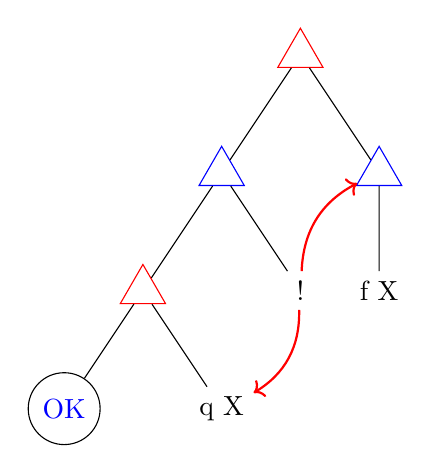
\begin{tikzpicture}[sibling distance=2cm]
  \node[draw,orNode] (A) {\orN}
    child {  node[draw,andNode] (X) {\andN}
      child { node[draw,orNode] (D) {\orN} 
        child { node[okNode]  {OK} }
        child { node (KILL) {q X} }
      }
      child { node (CUT) {!} }
    }
    child { node[draw,andNode] (C) {\andN}
      child { node (B) {f X} }
    };
    % \draw[very thick,-{latex[length=2.5mm,width=2.5mm]},blue] (A)..controls +(south east:15cm) and +(south west:11cm)..(B);
    \draw[draw, thick, red, ->] (CUT) to[bend left] (C);
    \draw[draw, thick, red, ->] (CUT) to[bend left] (KILL);
\end{tikzpicture}

\end{document}